\chapterimage{unidades/2_informacion/1_bajo_nivel/imagenes/cover}
\chapterimagedescription{Fotografía artistica que representa información}
\chapterimageauthor{Fotografía de Pixabay}

\chapter{Bajo nivel}
\index{Bajo nivel}
\label{chap:bajo_nivel}

En este capítulo analizaremos como la computadora transmite y almacena
información, y como procesa los datos que tiene almacenados. También veremos
como la concepción de ``información'', independientemente del tipo de
información que se trate y que tan compleja sea, puede abstraerse a una
interpretación sencilla capaz de ser procesada rápida y eficazmente por una
computadora.

También veremos como las computadoras solamente trabajan con electricidad, y
como esta puede ser utilizada para representar todo tipo de información mediante
una codificación.

\section{Representación de Información}
\label{chap:bajo_nivel:sec:representacion_informacion}

¿Cómo hacen las computadoras para hacer todo lo que hacen? ¿Dónde guardan las
cosas? ¿Cómo saben? Son preguntas que en general el usuario promedio de
computadoras, no versado en la temática, suele hacerse en algún momento.

En esta sección intentaremos responder algunas de esas preguntas, analizando en
primer lugar la pregunta ``¿Qué es la información?'' desde la perspectiva de una
computadora. Tras contestar eso veremos como estas complejas máquinas pueden
procesar esa información para realizar diversas tareas.

Esto nos llevará a sumergirnos aún más en el mundo del software y en su
interacción con el hardware en el nivel más sencillo, para luego ascender en un
proceso espiral en los distintos niveles de abstracción que existen en el
software.

\subsection{Códigos y comunicación}
\label{chap:bajo_nivel:subsec:codigos}

\index{Comunicacion@Comunicación}
Olvidemonos de las computadoras solo por un momento y empecemos por analizar un
poco la comunicación humana. Digamos que queremos comunicarnos con alguien, por
ejemplo, hablando. Nosotros seríamos entonces el \textbf{emisor} de la
comunicación, y la persona con la que hablamos el \textbf{receptor}. Además, la
comunicación se produce siempre mediante un \textbf{canal}, es decir, un medio
físico capaz de transferir la información desde el emisor hasta el receptor (en
el caso del habla, el canal es el aire, capaz de propagar las ondas sonoras).
Por el canal circula el \textbf{mensaje}, que es el elemento de la comunicación
que se transfiere desde el emisor hacia el receptor (en el caso del habla, las
ondas sonoras).

Ahora bien, no haga trampa y no se adelante en el texto, lea solo lo que tiene
inmediatamente a continuación, y responda ¿Puede descifrar el siguiente mensaje
alienígena?

\centerline{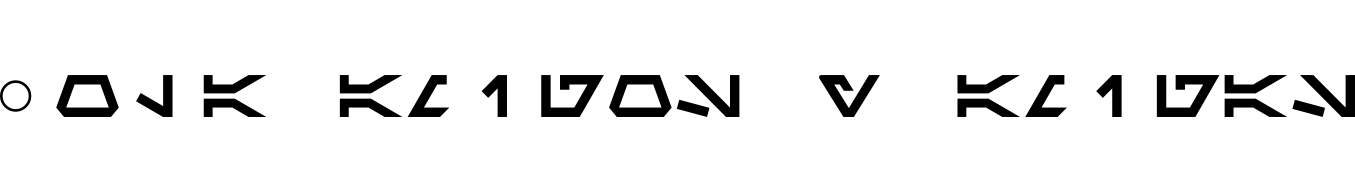
\includegraphics[]{unidades/2_informacion/1_bajo_nivel/imagenes/secret_message_A1.png}}

Lo más probable es que la respuesta sea que no. Aquí va una pista, cada símbolo
que aparece en el mensaje corresponde a una letra. ¿Puede descifrarlo ahora?.
¿Todavía no? Muy bien, la respuesta era:

\centerline{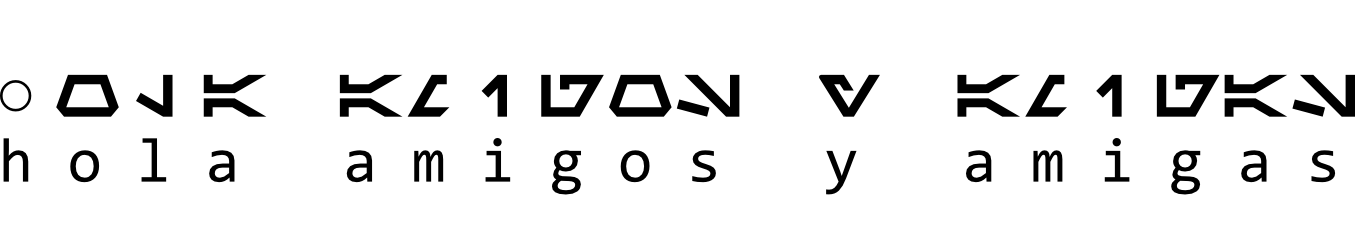
\includegraphics[]{unidades/2_informacion/1_bajo_nivel/imagenes/secret_message_A2.png}}

¿Lo intentamos una vez más? Intente descifrar ahora este mensaje:

\centerline{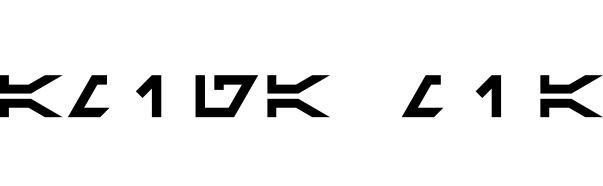
\includegraphics[]{unidades/2_informacion/1_bajo_nivel/imagenes/secret_message_B1.png}}

¿Lo logró? Debería haberle sido más sencillo. El mensaje era ``amiga mía''. El
truco estaba en buscar el mismo símbolo en el mensaje anterior, y luego ir
reemplazando cada símbolo con la letra correspondiente.

\centerline{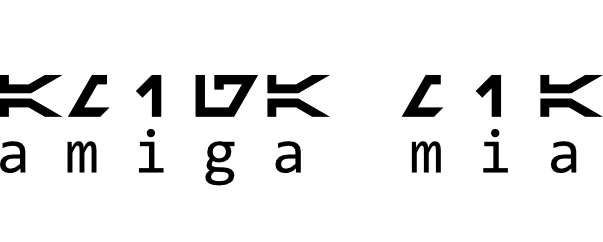
\includegraphics[]{unidades/2_informacion/1_bajo_nivel/imagenes/secret_message_B2.png}}

Si colocáramos cada símbolo junto a su correspondiente letra, y lo hacemos para
todas las letras del abecedario, entonces tendríamos una simple tabla que nos
permitiría no solo leer cualquier mensaje que use esos símbolos, sino también
escribir mensajes con los mismos.

Esta práctica es algo común que muchos realizamos cuando éramos chicos, como
parte de un juego que nos permitía enviarle mensajes secretos a otra persona,
sin que terceros (por ejemplo, nuestros padres, o las maestras) pudieran
leerlos. El truco consistía en que la tabla de símbolos solo fuera conocida por
nosotros y por la persona a quien le íbamos a enviar los mensajes.

Imaginemos ahora dos barcos que se cruzan en alta mar en la noche. Los barcos se
encuentran lo suficientemente lejos como para que el sonido de la voz de sus
capitanes viaje de un barco a otro, pero sin embargo están lo suficientemente
cerca como para ver las luces del otro barco. Así, si los capitanes desean
comunicarse, pueden usar la luz (por ejemplo, de una linterna) como canal de
comunicación. Un capitán puede enviar mensajes mediante una serie de parpadeos
lumínicos que genera con su linterna (los cuales pueden ser largos o cortos) y
que el otro capitán podría entender. Pero, para poder comunicarse efectivamente,
ambos capitanes deben tener una serie de reglas o convenciones en común que le
permitan saber que significan dichos parpadeos. Un parpadeo corto y uno largo,
fácil, la letra ``A'', uno corto, uno largo y luego dos cortos, la letra ``L''.

Este sistema ideado por Samuel F.B. Morse en 1836, para ser utilizado en
sistemas telegráficos. En general las personas que utilizan código Morse no
hablan de parpadeos lumínicos largos y cortos, sino de ``rayas'' y ``puntos'',
pues es una convención sencilla para escribir esos parpadeos. Si deseamos
comunicarnos basta tener la siguiente tabla a mano:

\vspace{0.5cm}
\centerline{
    \begin{tabular}{l l | l l | l l }
        letra & código & letra & código & letra & código \\
        \hline
        A & $\cdot -$                 & J & $\cdot - - -$         & S & $\cdot
        \cdot \cdot$\\
        B & $- \cdot \cdot \cdot$     & K & $- \cdot -$           & T & $-$\\
        C & $- \cdot - \cdot$         & L & $\cdot - \cdot \cdot$ & U & $\cdot
        \cdot -$\\
        D & $- \cdot \cdot$           & M & $- -$                 & V & $\cdot
        \cdot \cdot -$\\
        E & $\cdot$                   & N & $- \cdot$             & W & $\cdot -
        -$\\
        F & $\cdot \cdot - \cdot$     & O & $- - -$               & X & $- \cdot
        \cdot -$\\
        G & $- - \cdot$               & P & $\cdot - - \cdot$     & Y & $- \cdot
        - -$\\
        H & $\cdot \cdot \cdot \cdot$ & Q & $- -\cdot -$          & Z & $- -
        \cdot \cdot$\\
        I & $\cdot \cdot$             & R & $\cdot - \cdot$       & \\
    \end{tabular}
}

En el caso de los mensajes alienígenas y el juego que realizábamos cuando chicos
era que el sistema de reglas que usábamos para leer y escribir el mensaje es
secreto, solo nosotros y alguien más lo conocía. En el caso del código Morse en
cambio, el código no debe ser secreto, sino todo lo contrario (todos los
capitanes de barcos deberían saberlo para que podamos comunicarnos
efectivamente).
\autocite{petzold_2000}

\begin{definition}\index{Codigo@Código} Un \textbf{código} es un sistema de
    reglas que permiten convertir información dada por el emisor de un mensaje
    en alguna forma (letras, símbolos, gestos, parpadeos lumínicos, sonidos u
    otros) en información relevante para el receptor (probablemente en otra
    forma).
\end{definition}

Pero, que tiene todo esto que ver con las computadoras. Para eso debemos
mantener esta idea en la cabeza unos minutos mientras analizamos un poco el
hardware de la computadora.

\subsection{Electricidad y cables}
\index{Electricidad}\index{Cables}

Las computadoras modernas son dispositivos principalmente electrónicos, por
tanto solamente pueden manipular la electricidad que fluye por sus cables
(principalmente de cobre, como los de las instalaciones eléctricas, pero de
tamaños mucho más reducidos y con mucha menos carga eléctrica). La computadora
posee una serie de dispositivos que bloquean o no el paso de corriente eléctrica
en determinados casos (similar a un interruptor eléctrico, pero que no requiere
de intervención mecánica) llamados transistores. También existen en la
computadora otra serie de dispositivos electrónicos como resistencias,
capacitores, osciladores, etc. Estos se combinan de intrincadas formas para
permitir o no el paso de electricidad en determinados cables ante ciertas
condiciones, formando lo que conocemos como \textbf{circuitos}.

\begin{definition}\index{Circuito Elctronico@Circuito Electrónico} Un
    \textbf{circuito electrónico} consiste en un conjunto de componentes
    electrónicos, tales como resistencias, transistores, capacitores, inductores
    y diodos, conectados mediante cables o trazas conductivas a través de los
    cuales fluye corriente eléctrica.
\end{definition}

Todas las cuentas y cálculos que la computadora realiza, todas las imágenes que
se muestran en pantalla, todo es solamente electricidad. Así \textbf{los cables
de la computadora son el canal por el que fluye la comunicación}, mientras que
\textbf{la electricidad que fluye por los cables conforma el mensaje}.

Si queremos comunicarnos con una computadora debemos pensar en el proceso
comunicacional que ocurre. El emisor y el receptor alternan entre usuario y
computadora, ya sea que el usuario ingrese datos a esta, esta le brinde
información al usuario. Más importante es pensar en el canal y en el mensaje de
dicha comunicación.

El único canal existente son los cables que mencionamos, y el mensaje solo puede
estar dado por pulsos eléctricos. Muy similar al ejemplo de las linternas, donde
solo teníamos ``puntos'' o ``rayas'', aquí solo tenemos electricidad enviada por
un cable (o no enviada). Es decir, en un único cable, hay solo dos posibles
mensajes en un mismo momento.

Podemos decir que nuestros mensajes están limitados al canal en donde se
transmite. Si consideramos más cables, veremos que podemos enviar electricidad
por algunos de ellos, mientras que no lo hacemos por otros, dando lugar a una
mayor cantidad de combinaciones, que aumenta exponencialmente a medida que
agregamos cables. Esto permite enviar combinaciones más complejas, y por tanto
mayor cantidad de mensajes en un mismo momento. Nos centraremos más en esto en
las siguientes secciones, pero tenga en cuenta el lector que en general, no nos
interesa analizar un único cable, sino varios de ellos, pues es cuando se
combinan de diversas formas que efectivamente se tiene información interesante.

Siguiendo con los circuitos, los mismos \textbf{pueden tener formas sumamente
complejas que permiten realizar operaciones de lo más variado, como sumas,
restas, multiplicaciones y demás}. De esta forma, la información que ingresamos
puede ser procesada para transformarse en información que la computadora nos
brindará luego.\autocite[cap. 1]{nisan_2005}

Uno de los principales problemas que tienen los circuitos hechos con
transistores y cables, es que solo funcionan mientras hay electricidad. Si por
ejemplo, se cortara el suministro eléctrico todo lo que hay en la computadora se
pierde. Sin embargo, es deseable almacenar información para un uso posterior
(por ejemplo, guardar una imagen o un video digital). Así, existen dispositivos
que utilizan otros elementos para almacenar información, conocidos como
\textbf{periféricos de almacenamiento}. Todos estos dispositivos son capaces de
tomar la electricidad que circula por un cable especifico (conjunto de cables en
realidad, aunque no nos centraremos aquí en el funcionamiento detallado de los
dispositivos) y almacenarla de alguna forma tal que luego pueden leer y
transformar nuevamente en pulsos eléctricos que viajan por dicho cable.

Los discos rígidos son un ejemplo de periférico de almacenamiento que utilizan
una serie de imanes microscópicos que pueden estar orientados hacia alguna de
dos direcciones posibles. El disco contiene un cabezal que puede leer la
dirección a la que apunta un imán particular, o alterarla. Si lee una cierta
dirección, el dispositivo es capaz de mandar un pulso eléctrico (usando energía
que proviene de la fuente de alimentación) por alguno de los cables relevantes.

Los discos ópticos (CD/DVD) operan de forma similar, pero con una superficie que
refracta la luz, un láser y sensores ópticos en lugar de imanes y un cabezal.
Dependiendo del lugar hacia donde se refracte la luz, el dispositivo enviará
pulsos eléctricos en determinados cables.

Las tarjetas perforadas hacen algo parecido con punciones sobre una superficie
de cartón o papel, para que luego un cabezal intente pasar por un determinado
lugar de la tarjeta, trasmitiendo electricidad si se encontraba perforada en ese
lugar, pero bloqueando el paso de la misma si no lo estaba.

De esta forma, podemos decir que, \textbf{todo la información en una computadora
(es decir, el software) no es más que electricidad pasando por cables,
transistores y resistencias que se unen en formas extremadamente complejas,
formando circuitos, que permiten procesar datos y comunicarse entre usuario y
máquina}.\autocite[part. 2]{white_2015}


\subsection{Código Binario}
\index{Codigo Binario@Código Binario}\index{Binario}
\label{chap:bajo_nivel:subsec:binario}

Imaginemos un conjunto de ocho (8) cables. El pasaje o no pasaje de electricidad
por dichos cables hace finalmente al mensaje. Probablemente nos interese
mencionar en algún momento, por qué cables pasa electricidad y por cuales no,
para determinar cuál es el mensaje que estamos, o bien enviando a la máquina, o
bien recibiendo de ella. Podríamos graficar nuestros cables de la siguiente
forma:

\centerline{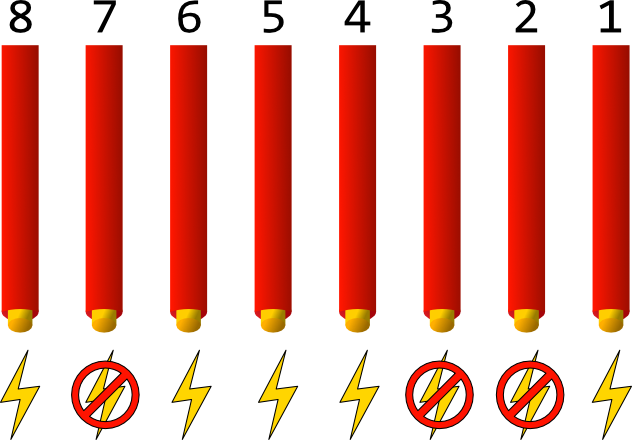
\includegraphics[]{unidades/2_informacion/1_bajo_nivel/imagenes/cables_electricity.png}}

En este caso numeramos los cables del 0 al 7 de derecha a izquierda (podríamos
haber numerado del 1 al 8 y de izquierda a derecha. La elegida es una convención
arbitraria, pero útil en términos prácticos y por tanto, muy utilizada). Como se
puede predecir, cuando la cantidad de cables aumenta de unos pocos a cientos, a
miles, realizar un dibujo para indicar en qué cables pasa electricidad y en
cuáles no deja de ser viable.

\begin{knowwhat}[En realidad]
En realidad, los cables siempre tienen electricidad, pero el voltaje que pasa
por los mismos es distinto. Los circuitos se ``activan'' cuando el nivel de
voltaje supera un umbral (por ej. 1.5 voltios), por lo que todo cable por el que
pase menos voltaje se considera ``apagado'' y por el que pase más ``encendido''.
\end{knowwhat}

Así es como surge la idea de utilizar alguna especie de \textbf{código} para
poder hablar del mensaje que se transmite por esos cables, sin tener que
realizar complejos dibujos o diagramas. Esto nos permite además abstraernos de
los cables y circuitos, es decir, del canal, para centrarnos en el mensaje.

\index{Codigo Binario@Código Binario}\index{Sistema Binario}\index{Binario} El
código elegido para representar el estado de los cables internos de la
computadora es el \textbf{código binario}, o lo mismo el \textbf{sistema
binario}. El \textbf{sistema binario} es un sistema numérico en el que solamente
se utilizan dos símbolos, \textbf{cero} y \textbf{uno} (nuevamente, una
convención, cualquier otro par de símbolos, ej. ``A'' y ``B'' hubiera sido
perfectamente válido). Así, un \textbf{número binario} se compone de una
secuencia de ceros y unos (Por ej. 10100111). Como el sistema solo permite dos
números, es ideal para representar los estados de los cables en la computadora
que trabajan con presencia o ausencia de electricidad. Por lo tanto, podríamos
representar el estado de nuestros ocho cables con un número.

\centerline{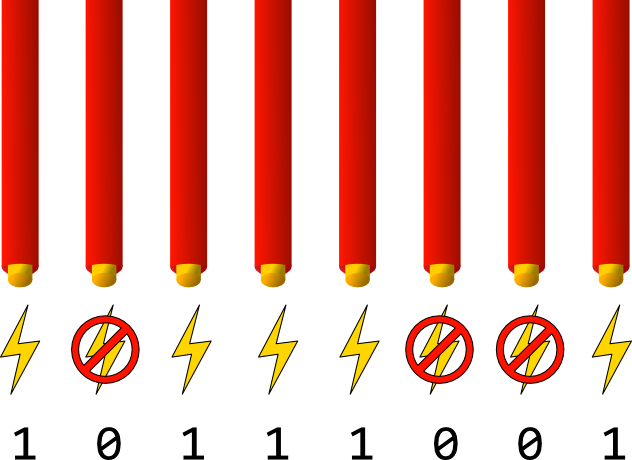
\includegraphics[]{unidades/2_informacion/1_bajo_nivel/imagenes/binary_cables_electricity.png}}

En este caso, elegimos que el dígito 1 representa la presencia de electricidad,
mientras que el 0 representa su ausencia, pero podría haberse elegido de forma
inversa, es irrelevante, pues es solo una convención.

\begin{definition}\index{Codigo Binario@Código Binario}\index{Sistema
    Binario}\index{Binario} El \textbf{sistema binario} es un sistema numérico
    posicional de dos dígitos, los cuales son en general representados mediante
    cero y uno (0 y 1).\autocite{laplante_2000}
\end{definition}

Como ya vimos en la sección anterior, la electricidad que fluye por los cables
puede eventualmente almacenarse en un dispositivo adicional, como un disco
rígido, que utiliza imanes para representar la presencia o ausencia de
electricidad. Si almacenamos en un disco, podríamos representarlo gráficamente
de la siguiente forma:

\centerline{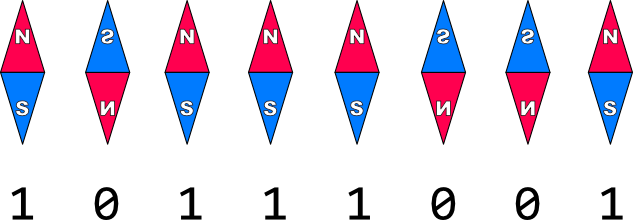
\includegraphics[]{unidades/2_informacion/1_bajo_nivel/imagenes/binary_magnets.png}}

Como vemos, el número binario que representa al valor almacenado es el mismo que
el que representa a la electricidad en los cables. Podríamos ver que esto aplica
también en otros dispositivos de almacenamiento, como por ejemplo, las tarjetas
perforadas:

\centerline{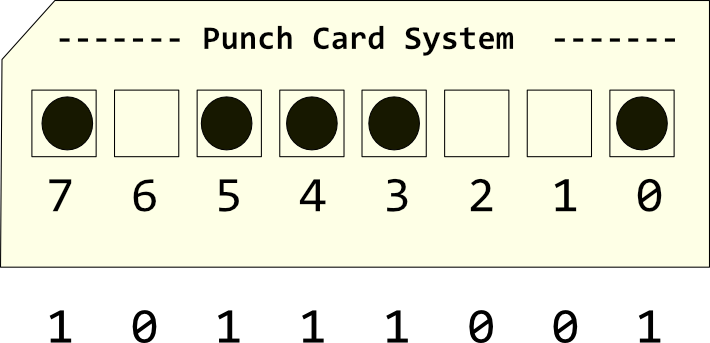
\includegraphics[]{unidades/2_informacion/1_bajo_nivel/imagenes/binary_punchcard.png}}

\textbf{El sistema binario es lo suficientemente versátil para permitirnos
hablar acerca de lo que vamos a almacenar o transmitir por un cable, sin
importar el medio físico subyacente. Así, nos permite abstraernos del
dispositivo y pensar acerca de la información que fluye en la computadora de
forma matemática.}

El sistema binario fue estudiado por primera vez en el siglo III A.C. por el
matemático indio Pingala, coincidiendo con el descubrimiento del concepto del
número cero. El matemático alemán Leibniz documentó en su totalidad el sistema
en el siglo XVII, en su artículo ``Explication de l\'Arithmétique Binaire''. En
1854, el matemático británico George Boole publicó un artículo que marcó un
antes y un después, detallando un sistema de lógica que terminaría denominándose
``Álgebra de Boole''. La elección de este sistema para representar los datos
responde entonces también a la gran cantidad de documentación y trabajos previos
sobre dicho sistema numérico.

\subsection{Codificación de información}
\index{Codificacion@Codificación}\index{Informacion@Información}
\label{chap:bajo_nivel:subsec:codificacion}

Vamos a realizar un juego, similar al que hicimos dos secciones atrás. ¿Se anima
a descifrar este mensaje?

\centerline{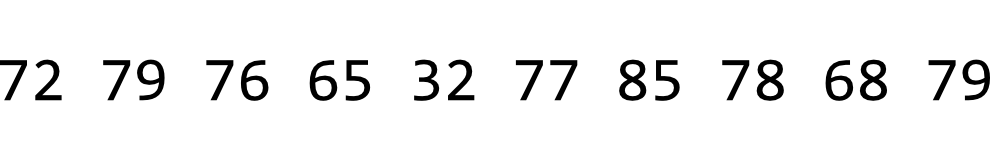
\includegraphics[]{unidades/2_informacion/1_bajo_nivel/imagenes/ascii_message_A.png}}

Por supuesto que a priori es imposible identificar el mensaje, pero si seguimos
la misma lógica de antes, podríamos asignar un número a cada letra, y
obtendríamos una tabla que nos permita realizar la conversión de uno a otro. Es
decir, sabemos que para poder entender ese mensaje, necesitamos un
\textbf{código}. Dado el código en la siguiente tabla:

\centerline{
    \begin{tabular}{l l | l l | l l }
        letra & número & letra & número & letra & número \\
        \hline
        A & 65 & J & 74 & S & 83\\
        B & 66 & K & 75 & T & 84\\
        C & 67 & L & 76 & U & 85\\
        D & 68 & M & 77 & V & 86\\
        E & 69 & N & 78 & W & 87\\
        F & 70 & O & 79 & X & 88\\
        G & 71 & P & 80 & Y & 89\\
        H & 72 & Q & 81 & Z & 90\\
        I & 73 & R & 82 & espacio & 32 \\
    \end{tabular}
}

¿Ahora puede identificar el mensaje dado? Claro que si, es cuestión de
reemplazar uno a uno los número por las letras dadas.

\centerline{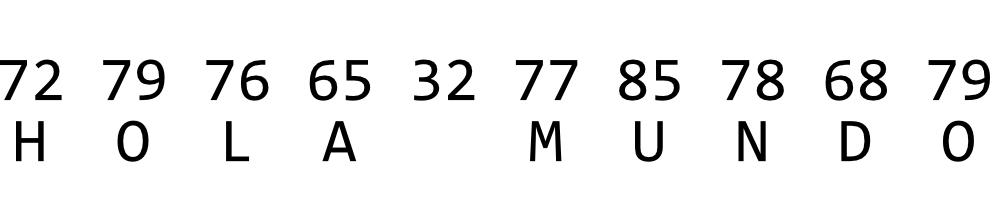
\includegraphics[]{unidades/2_informacion/1_bajo_nivel/imagenes/ascii_message_B.png}}

Imagínese ahora que la tabla no la tenemos solo dos personas, sino que es una
tabla que todo el mundo conoce, y a la que todo el mundo tiene acceso. Si ese
fuera el caso, entonces cualquier persona podría escribir un mensaje en forma de
números, y cualquiera podría leerlo.

Más interesante aún, podríamos representar otras cosas que no sean letras como
números, o como grupos de números, por ejemplo, colores:\autocite{msx_1985}

\centerline{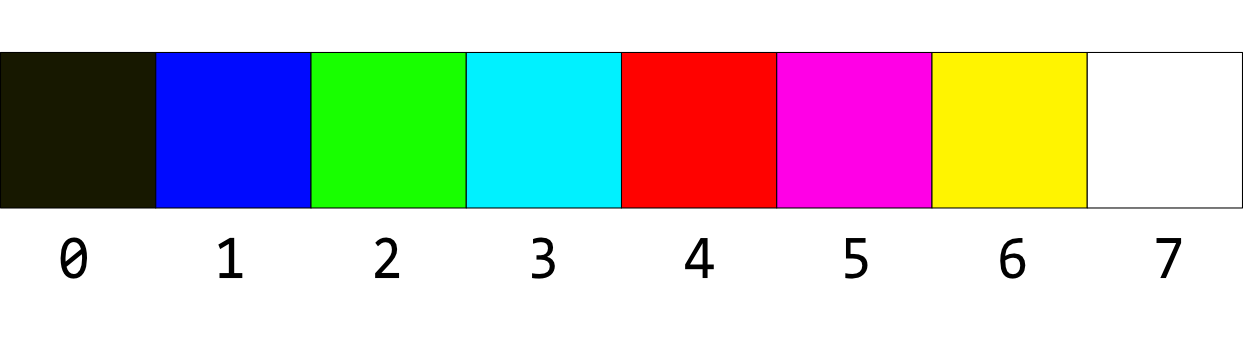
\includegraphics[scale=0.8]{unidades/2_informacion/1_bajo_nivel/imagenes/palette_3bits.png}}

Teniendo colores, podríamos representar una imagen como una secuencia de
números.

\centerline{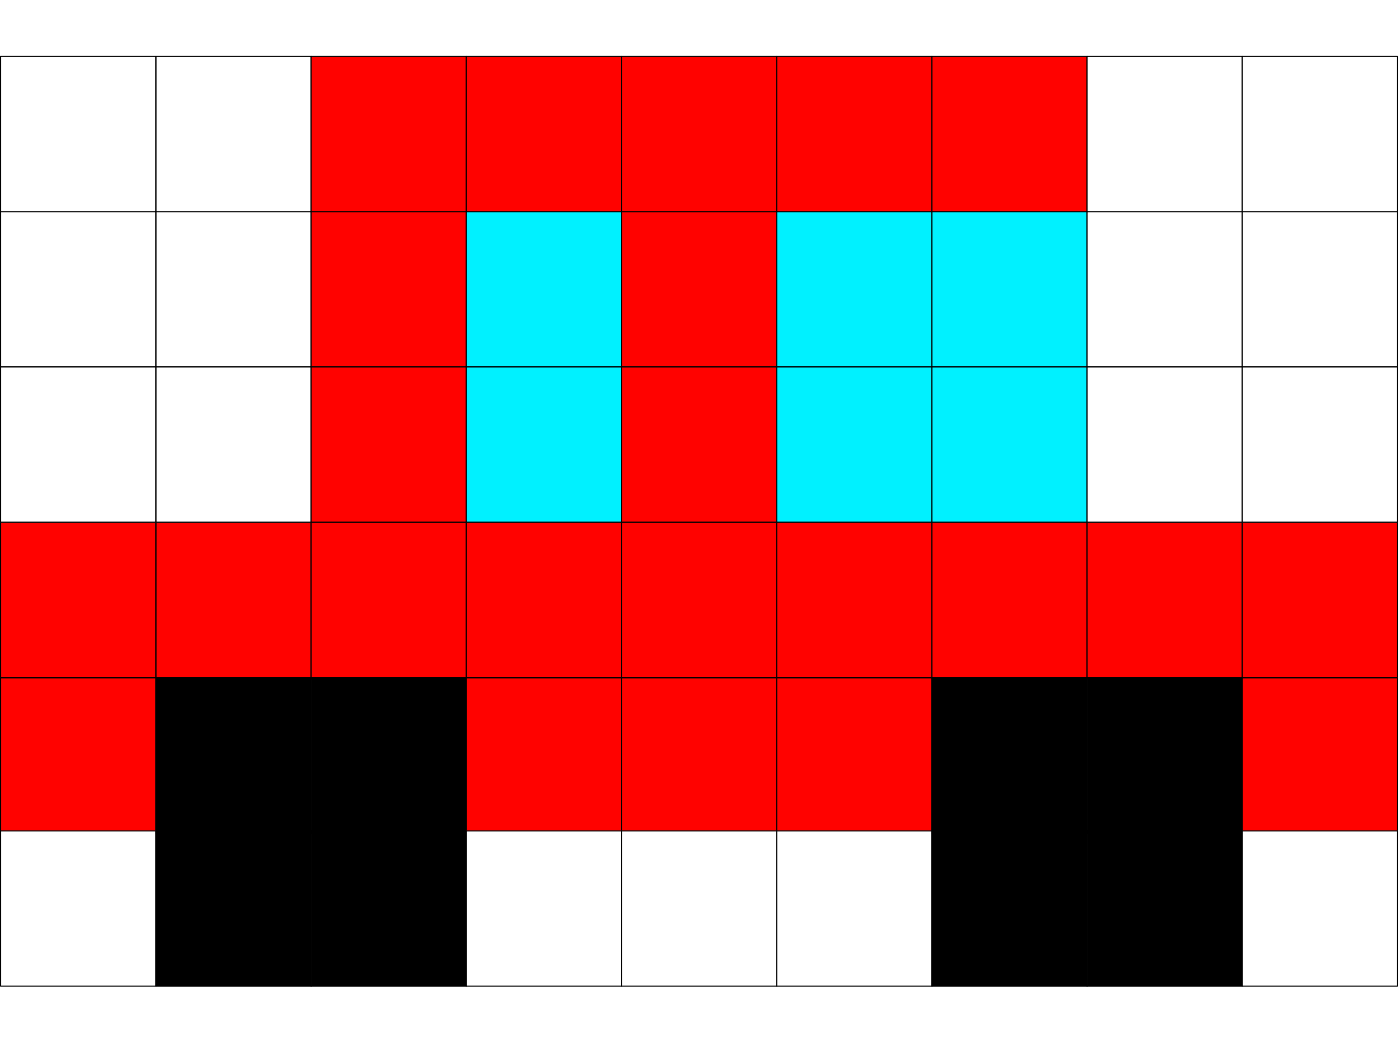
\includegraphics[scale=0.75]{unidades/2_informacion/1_bajo_nivel/imagenes/pixels_car.png}}

Para representar una imagen, la misma debe ser dividida en una grilla
cuadriculada en donde cada celda tiene un único posible color. Luego podemos
determinar el color de cada celda haciendo un reemplazo uno a uno con la
representación de colores que vimos anteriormente, para obtener una secuencia de
números. Además deberíamos indicar el alto y el ancho de la imagen, y elegir el
orden en el que vamos a leer la secuencia (por ejemplo, de izquierda a derecha y
de arriba a abajo).

\centerline{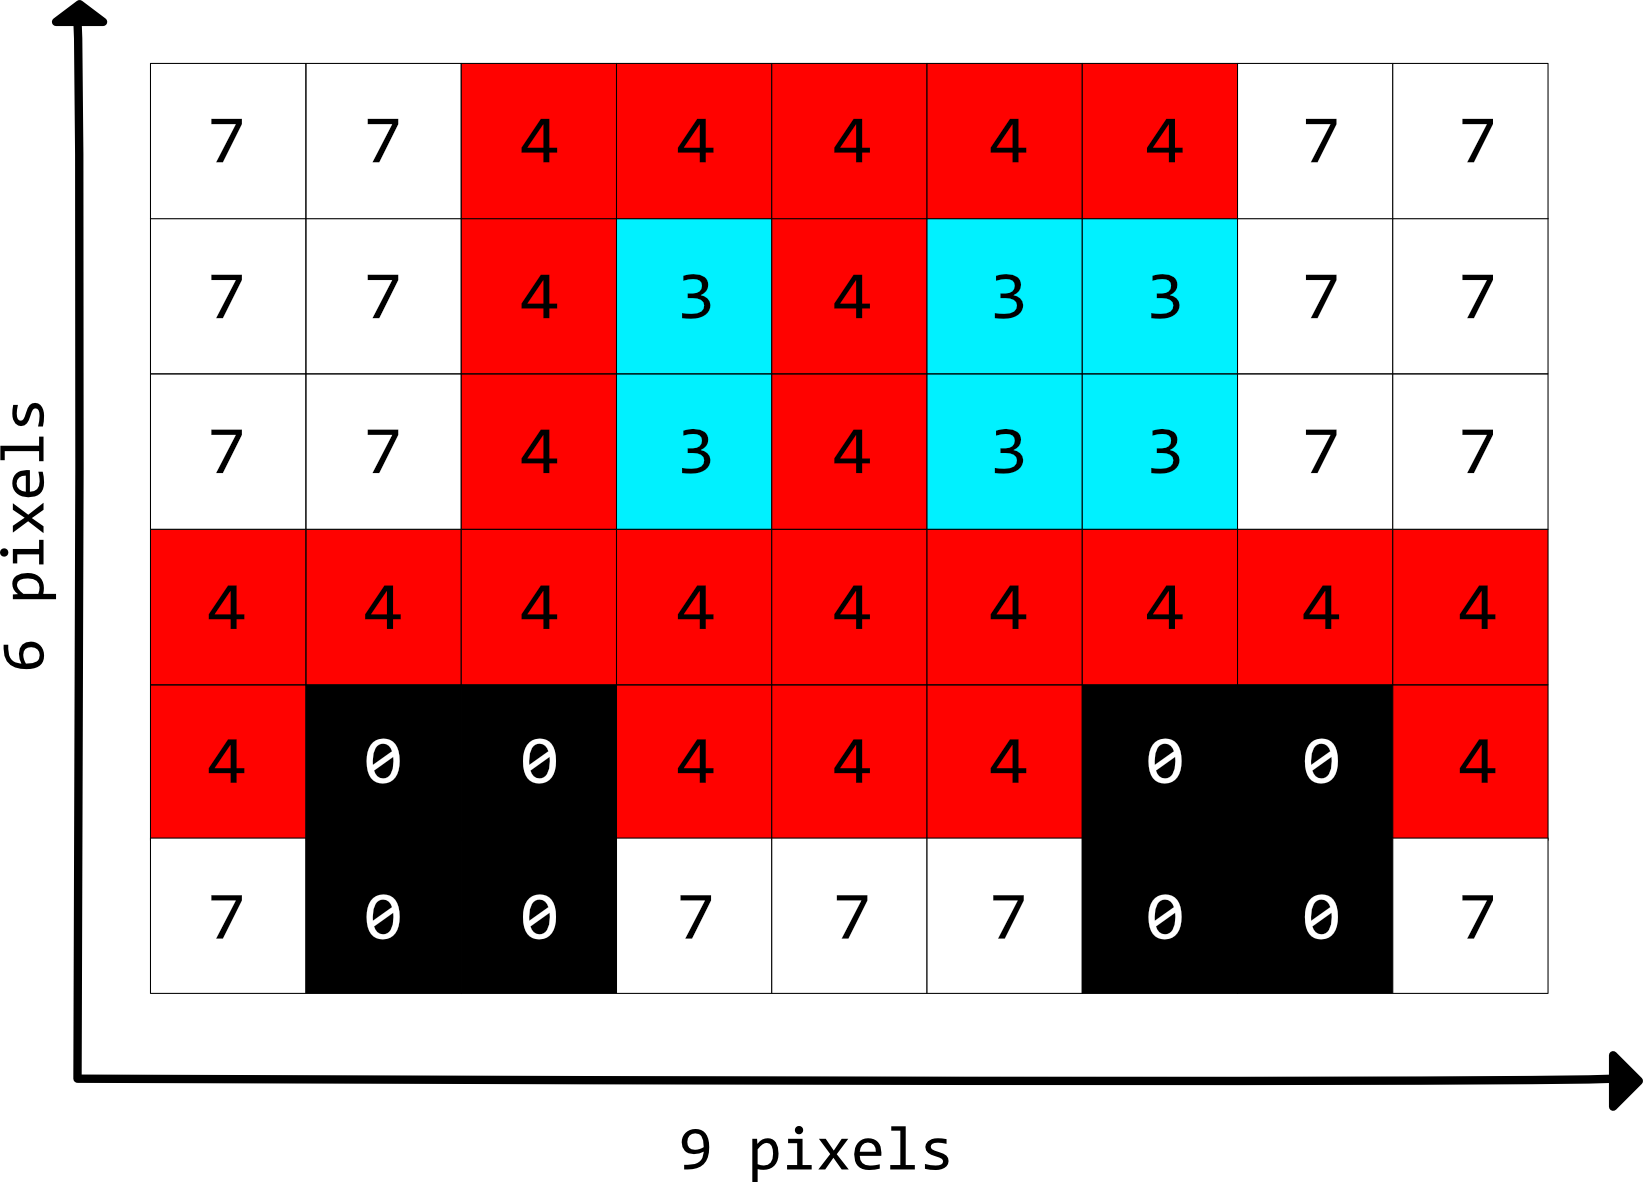
\includegraphics[scale=0.75]{unidades/2_informacion/1_bajo_nivel/imagenes/pixels_car_labeled.png}}

Si tomamos los dos primeros dos dígitos como ancho y alto respectivamente, vemos
que se indica que la imagen tiene 9 celdas de ancho, por 6 de alto. El resto
corresponde a cada uno de las celdas de la grilla, indicando para cada una, que
color tiene.

\centerline{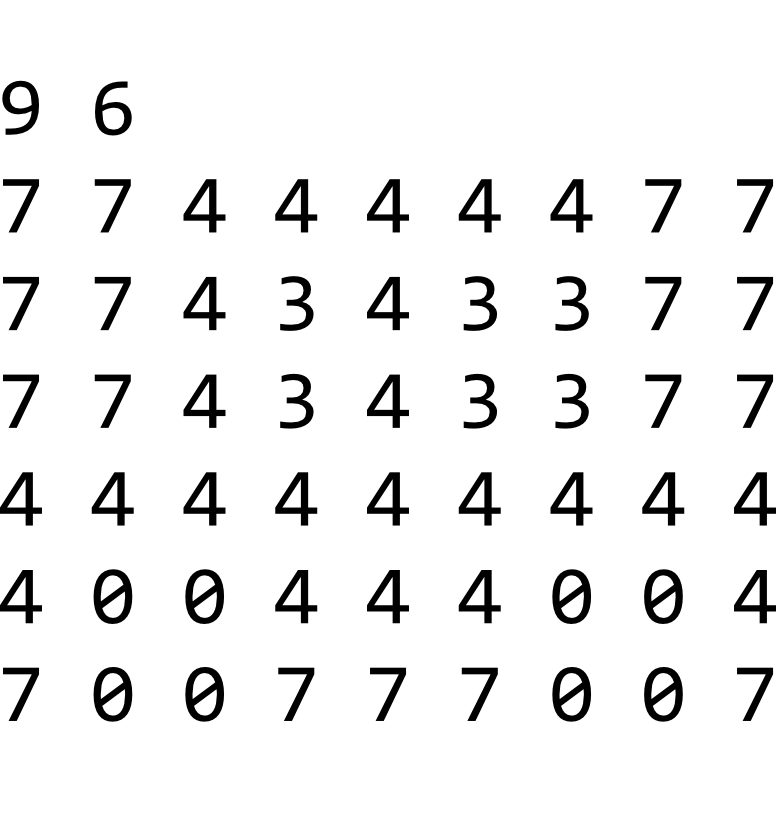
\includegraphics[]{unidades/2_informacion/1_bajo_nivel/imagenes/pixels_car_numbers.png}}

Dispusimos los números en forma de filas y columnas, similar a la imagen, para
que sea fácil de leer, pero esto no es necesario. Más aún, como cada color se
compone solo de un dígito, podemos eliminar completamente los espacios entre un
dígito y otro, transformando nuestra imagen en un gran número.

\centerline{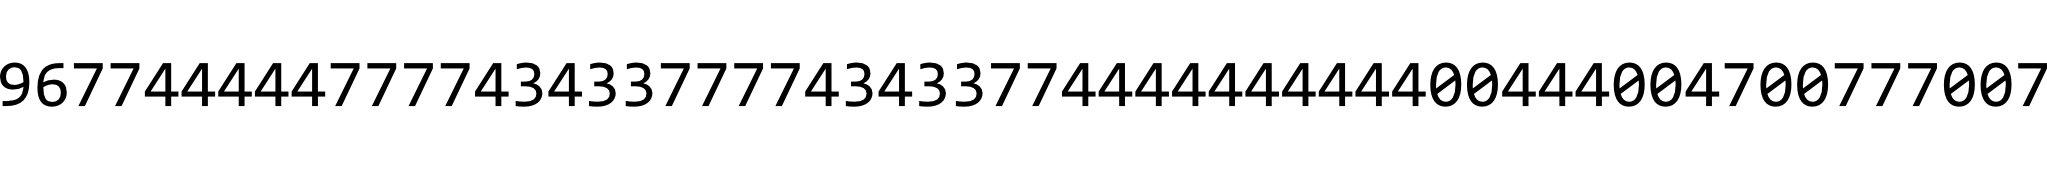
\includegraphics[]{unidades/2_informacion/1_bajo_nivel/imagenes/pixels_car_numbers_final.png}}

Note que el ancho y el alto no deben ser superiores a 10, para que efectivamente
sea entendible por el receptor.

\begin{definition}\index{Codificacion@Codificación} Se conoce como
    \textbf{codificación} al proceso mediante el cual una cierta información
    (por ejemplo, una imagen, un color, una letra) es transformada en algún otro
    elemento que la representa mediante la utilización de un código. El proceso
    inverso se conoce como \textbf{decodificación}.
\end{definition}

\image{unidades/2_informacion/1_bajo_nivel/imagenes/resolution.png}
{Ejemplo de como la calidad de imagen aumenta a medida que aumenta su
resolución.} {Imagen de dominio público.}

\begin{knowwhat}
Las pantallas de los monitores, celulares y otros dispositivos electrónicos
están compuestas de cientos de miles de pequeñísimos puntos conocidos como
\textbf{pixeles}. Cada \textbf{pixel} puede prenderse de un único color (o estar
apagado y verse negro). Las imágenes digitales entonces se almacenan guardando
la información de que color debe tener cada pixel.

Los sensores de las cámaras digitales funcionan igual. La cantidad de sensores
se mide en \textbf{megapixeles} y tiene que ver con la cantidad de puntos que
van a conformar la imagen.

Las imágenes digitales entonces se almacenan basados en los pixeles, aunque como
la cantidad de sensores de la cámara y la cantidad de puntos en la pantalla no
siempre coincide, a veces un único pixel de una imagen puede corresponder a
varios puntos de la pantalla. La cantidad de pixeles que tiene una imagen es lo
que se conoce como \textbf{resolución} de la imagen. A mayor resolución, más
nítida y de mejor definición, a costa de que ocupa mayor espacio de
almacenamiento.
\end{knowwhat}

Es decir, cualquier tipo de elemento del que podamos querer hablar es
susceptible de ser codificado mediante números.\autocite[p. 16]{white_2015} Pero
eso es solo el principio de un proceso que va más allá, pues todo número puede
ser representado mediante binario.

\subsection{Representando números con binario}
\index{Numeros@Números}\index{Binario}
\label{chap:bajo_nivel:subsec:numeros}

El poder representar todo con números es una excelente idea, pero surge un
problema al querer guardar esos números en una computadora. Como ya vimos, la
computadora solo maneja unos y ceros (o electricidad y no electricidad), no
números naturales como los que necesitamos para representar nuestras letras,
colores e imágenes.

Por suerte, los números naturales pueden expresarse en binario con poco
esfuerzo. El truco consiste en elegir una representación binaria distinta para
cada número, de forma similar a lo que hicimos con las letras. Debemos para ello
partir de la cantidad de cables que vamos a tener, por ejemplo, ocho cables.
Luego, basta analizar todos los posibles estados en los que puede llegar a estar
ese conjunto de cables (por ejemplo, todos sin electricidad, todos con
electricidad, todos menos el último sin electricidad, todos menos los dos
últimos sin electricidad, y así siguiendo). Es decir, analizamos todos los
posibles números binarios que representarían a nuestro conjunto de cables.
Luego, basta asignar un número a cada binario. Por ejemplo, si tuviéramos cuatro
cables tendríamos:

\centerline{
    \begin{tabular}{l l | l l}
        número & binario &  número & binario \\
        \hline
        0 & 0000 & 8  & 1000 \\
        1 & 0001 & 9  & 1001 \\
        2 & 0010 & 10 & 1010 \\
        3 & 0011 & 11 & 1011 \\
        4 & 0100 & 12 & 1100 \\
        5 & 0101 & 13 & 1101 \\
        6 & 0110 & 14 & 1110 \\
        7 & 0111 & 15 & 1111 \\
    \end{tabular}
}

Note como la cantidad de cables que tenemos limita la cantidad de números que
podemos representar, siendo mayor los números a mayor cantidad de cables. En
particular:

\begin{equation}
    2^{\text{cant. cables}} = \text{cant. números distintos}
\end{equation}

Por supuesto no es la única representación posible, podríamos haber elegido
asignar los números en otro orden. Existen diferentes formas estandarizadas para
representar un número en binario, que incluso sirven para números negativos o
racionales, algo que no analizaremos pues escapa a los alcances del presente.

Lo importante es que \textbf{a toda representación numérica, se puede asignar
una representación binaria}. Así \textbf{toda la información digital, ya sea
texto, colores, o imágenes, pueden representarse con binario}.\autocite[p.
17]{white_2015}

Una secuencia de números se traduce entonces directamente a una secuencia de
números binarios, es decir, a una larga tira de unos y ceros. Y por tanto,
cualquier información es posible de ser representada como datos binarios.

\subsection{Bits, Bytes y otros}
\index{Bit}
\label{chap:bajo_nivel:subsec:bits}

Cuando se utilizan los unos y ceros para representar información se habla de
\textbf{bits}.

\textbf{Un bit es un dígito en el sistema de numeración binario}. Es decir,
corresponde a un único cero o uno en una posición determinada. \textbf{Si
tenemos un dato que está representado por ocho cables (o imanes, o lo que fuera)
decimos que está representado por 8 bits.}

\index{Byte}
Era muy común que las antiguas computadoras trabajaran con 8 bits. Como era muy
común la medida de 8 bits para representar datos, surge la palabra
\textbf{octeto} para indicar precisamente esa cantidad. Adicionalmente surge la
palabra \textbf{byte}. El \textbf{byte} suele representar 8 bits, pero en
algunas computadoras antiguas el término se utilizaba con otra acepción (por
ejemplo, 6, 7 o incluso 9 bits). Hoy en día la mayoría de las computadoras
hablan de \textbf{byte para referirse a 8 bits}.

\index{Kilobit}\index{Megabit}\index{Gigabit}\index{Terabit}\index{Petabit}\index{Exabit}
También es muy común escuchar los términos \textbf{kilobit} o \textbf{megabit}.
El prefijo corresponde a una escala adicional que indica una gran cantidad de
bits. Así de forma similar a como un kilometro representa mil metros, un kilobit
representa mil bits.

\begin{tabular}{l l l}
    Nombre   &  Prefijo  & Equivalencia\\
    \hline
    Kilobit  &  kbit     & 1000 bits \\
    Megabit  &  Mbit     & 1000 Kbits = 1.000.000 bits\\
    Gigabit  &  Gbit     & 1000 Mbits = 1.000.000.000 bits\\
    Terabit  &  Tbit     & 1000 Gbits = 1.000.000.000.000 bits\\
    Petabit  &  Pbit     & 1000 Tbit = 1.000.000.000.000.000 bytes\\
    Exabit   &  Ebit     & 1000 Pbit = 1.000.000.000.000.000.000 bytes\\
\end{tabular}

\index{Kilobyte}\index{Megabyte}\index{Gigabyte}\index{Terabyte}\index{Petabyte}\index{Exabyte}
Los bytes también son sujeto de los mismos prefijos, siendo un Kilobyte
equivalente a 1000 bytes.\autocite{laplante_2000}

\begin{tabular}{l l l}
    Nombre   &  Prefijo  & Equivalencia\\
    \hline
    Kilobyte  &  kB     & 1000 bytes = 8000 bits \\
    Megabyte  &  MB     & 1000 KB = 1.000.000 bytes\\
    Gigabyte  &  GB     & 1000 MB = 1.000.000.000 bytes\\
    Terabyte  &  TB     & 1000 GB = 1.000.000.000.000 bytes\\
    Petabyte  &  PB     & 1000 TB = 1.000.000.000.000.000 bytes\\
    Exabyte   &  EB     & 1000 PB = 1.000.000.000.000.000.000 bytes\\
\end{tabular}

Para tener una idea de lo importante que son estas medidas, basta con acercarse
a un local de hardware para comprar algunos dispositivos. Las memorias de
computadoras (conocidas como RAM) tienen su capacidad de almacenamiento
expresadas en Gigabytes (GB), siendo hoy en día comunes las de 2, 4 y hasta 8
GB, aunque hay incluso de más. Los discos rígidos también tienen su capacidad
expresadas en GB, siendo comunes los de 250, 500, 750, e incluso hay algunos que
llegan a ser de 1 TB.

Al contratar un servicio de conexión a internet, la velocidad de conexión se
expresa en Megabits por segundo (Es decir, cuantos bits se pueden descargar en
un segundo) siendo comunes hoy en día conexiones de 2, 4, 10, 20 y hasta 50
Mbits por segundo.

A continuación se deja una idea de cuanta información (comparada con información
impresa) representa cada medida.

\small
\begin{tabular}{r c l}
    Número de bytes	& Múltiplo & Equivalencia aproximada\\
    \hline
                        1 &	1 B	    & Una letra.\\
                       10 & 10 B	& Una o dos palabras.\\
                      100 & 100 B	& Una o dos frases.\\
                    1.000 &	1 kB	& Una historia muy corta.\\
                   10.000 &	10 kB	& Una página de enciclopedia con un dibujo
                   simple.\\
                  100.000 & 100 kB	& Una fotografía de resolución mediana.\\
                1.000.000 & 1 MB	& Una novela.\\
               10.000.000 & 10 MB	& Dos copias de la obra completa de
               Shakespeare.\\
              100.000.000 & 100 MB	& Un estante de un metro lleno de libros.\\
            1.000.000.000 & 1 GB	& Una camioneta llena de páginas con
            texto.\\
        1.000.000.000.000 & 1 TB	& Páginas con texto elaboradas de 50.000
        árboles.\\
       10.000.000.000.000 & 10 TB	& La colección impresa de la biblioteca de
       EE.UU.\\
    1.000.000.000.000.000 & 1 PB	& Los datos que maneja Google cada hora.\\
1.000.000.000.000.000.000 & 1 EB	& Todos los datos en Internet para finales
de 2001.\\
\end{tabular}
\normalsize

\section{Sistemas de Caja Negra}
\index{Caja Negra}
\label{chap:bajo_nivel:sec:caja_negra}

En muchas ocaciones es útil pensar los sistemas como una \textbf{caja negra}. Es
decir, un elemento o proceso del cual no nos importa el funcionamiento interno,
pero si sabemos que, ante cierta entrada, producirá cierta salida.

\begin{definition}
    Se denomina \textbf{caja negra} a aquel elemento que es estudiado desde el
    punto de vista de las entradas que recibe y las salidas o respuestas que
    produce, sin tener en cuenta su funcionamiento interno.
\end{definition}

\image{unidades/2_informacion/1_bajo_nivel/imagenes/caja_negra.png}
{Ilustración de un proceso de Caja Negra.} {Ilustración propia.}

Puede pensarse una analogía al proceso de caja negra con un auto. Cualquier
persona puede conducir un auto. Basta comprender que, ante la presión del pedal
del acelerador, y habiendo colocado la palanca de cambios en la posición
correcta, el auto irá hacia adelante. Los funcionamientos internos del vehículo,
tales como los detalles sobre el funcionamiento de un motor de combustión
interna, la batería, o la caja de cambios, no son necesarios desde el punto de
vista del conductor.

En informática este proceso se debe llevar a cabo todo el tiempo, y en varios
niveles. Pensemos por ejemplo en el CPU, uno de los componentes de hardware más
complejos presentes en las computadoras modernas. El mismo está compuesto de
millones de transistores colocados e interconectados de intrincadas formas. Si
lo que nos interesa es diseñar microprocesadores, probablemente sea relevante
conocer los detalles sobre como un procesador está estructurado y compuesto. Sin
embargo, si lo que nos interesa es es componer los grandes componentes de
hardware, el procesador será un elemento más, y su interior no es relevante. Más
aún, los componentes de hardware no son relevantes si lo que interesa es
analizar el software de la computadora. Un último ejemplo podría ser la forma en
la que los datos están codificados, como binario, que no interesa si lo que
queremos es utilizar el equipo, por ejemplo, editando una imagen o escribiendo
un texto.

El concepto de caja negra utilizado en sistemas no debe confundirse con el
``cajanegrismo''; éste es un concepto vinculado a la sociología que hace
referencia al hecho de que las personas suelen olvidar el funcionamiento interno
de las cosas (generalmente nuevos dispositivos tecnológicos) a medida que se
familiarizan con ellos y terminan por asimilarlos como de uso cotidiano.

La principal diferencia entre ambos conceptos radica en que el \textbf{estudio
de un sistema como una caja negra es un proceso de abstracción}, mientras que el
``cajanegrismo'' es más bien un proceso de olvido.

Por lo tanto, \textbf{concebir al hardware o al software de la computadora como
una caja negra} puede ser útil desde el punto de vista de un programador o un
usuario. \textbf{La concepción de caja negra es una idea que aplica de forma
constante en las disciplinas informáticas}, y es un concepto recurrente ya que
se deben realizar abstracciones de forma constante.

\section{Actividades}
\label{chap:bajo_nivel:sec:actividades}

\begin{exercise}
Dada la imagen a continuación, exprésela como un único número utilizando la
misma codificación que se aplicó en este capítulo.

\centerline{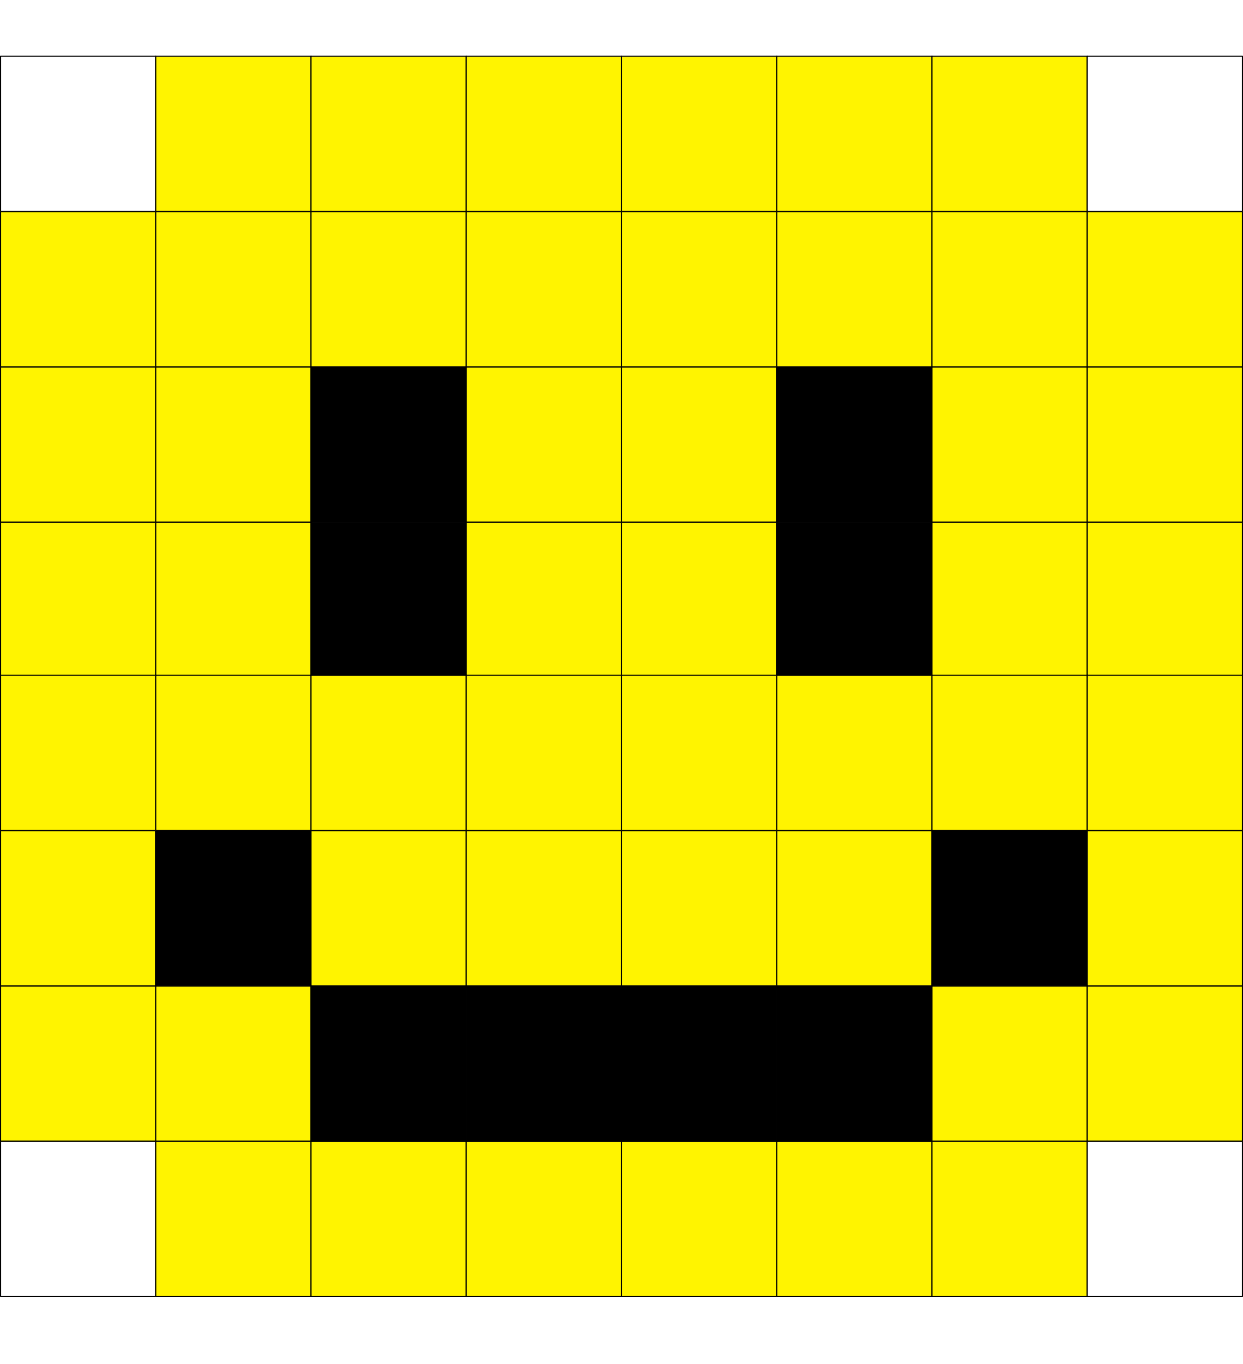
\includegraphics[scale=0.35]{unidades/2_informacion/1_bajo_nivel/imagenes/pixels_smile.png}}
\end{exercise}

\begin{exercise}
La tabla mostrada en este capítulo para representar letras como números
corresponde a la codificación ASCII. Utilizando esa tabla se pide que codifique
la siguiente frase como una serie de números.

\textbf{SOMOS LO QUE PROGRAMAMOS}
\end{exercise}

\begin{exercise}
Nuevamente, usando ASCII, se pide ahora que decodifique el siguiente mensaje
expresado como una serie de números.

\textbf{80 82 79 71 82 65 77 79 32 76 85 69 71 79 32 69 88 73 83 84 79}
\end{exercise}

\begin{exercise}
Si contamos con una computadora con 16 cables para representar nuestros datos,
¿Qué cantidad de números distintos pueden representarse con ellos?
\end{exercise}

\begin{exercise}
Un chiste de informáticos reza lo siguiente:

\textbf{``Solo hay 10 tipos de personas en este mundo, los que entienden binario
y los que no''}

En qué radica la gracia del chiste.
\end{exercise}
